\appendix

\section{Artifact description}

\subsection{Abstract}

Our research artifact consists of interactive Jupyter notebooks. For your convenience, we provide two methods of validating our results: an `AE' notebook which validates the main experiments of the paper, and a comprehensive `Paper' notebook which replicates every experiment of the paper, including additional analysis. The most convenient method to evaluate our results is to access our pre-configured live server:
\begin{verbatim}
http://[redacted]:8888/notebooks/AE.ipynb
\end{verbatim}
using the password \texttt{[redacted]}, and to follow the instructions contained within.

\subsection{Description}

\subsubsection{Check-list (Artifact Meta Information)}

{\small
  \begin{itemize}
    %   \item {\bf Program: }
    %   \item {\bf Compilation: }
    %   \item {\bf Transformations: }
    %   \item {\bf Binary: }
    %   \item {\bf Data set: }Default datasets for benchmarks.
    \item {\bf Run-time environment: }A web browser.% We tested with Google Chrome.
    %   \item {\bf Hardware: }None.
    %   \item {\bf Run-time state: }
    %   \item {\bf Execution: }
    \item {\bf Output: }OpenCL code, runtimes, figures and tables from the paper.
    \item {\bf Experiment workflow: }Run (or install locally) Jupyter notebooks; interact with and observe results.
    \item {\bf Experiment customization: }Edit code in Jupyter notebook; full API and CLI for CLgen.
    \item {\bf Publicly available?: }Yes, code and data. See:
    
    \url{http://chriscummins.cc/cgo17/}
  \end{itemize}
}

\subsubsection{How Delivered}

Jupyter notebooks which contain an annotated version of this paper, interleaved with the code necessary to replicate results. We provide three options to run the Jupyter notebooks:
\begin{enumerate}
  \item Remote access to the notebook running on our pre-configured experimental platform.
  \item Download our pre-packaged VirtualBox image with Jupyter notebook installed.
  \item Install the project locally on your own machine.
\end{enumerate}

\subsection{Installation}\label{subsec:installation}

Access the Jupyter notebooks using one of the three methods we provide. Once accessed, proceed to Section~\ref{subsec:workflow}.

\subsubsection{Remote Access}

The Jupyter notebooks are available at:

\url{http://[redacted]:8888}, password \texttt{[redacted]}.

\noindent
A dashboard showing server load is available at:

\url{http://[redacted]:19999}

\noindent
High system load may lead to inconsistent performance results; this may occur if multiple reviewers are accessing the server simultaneously.

\newpage
\subsubsection{Virtual Machine}

Copy our pre-configured 5.21 GB VirtualBox image using:
\begin{verbatim}
$ scp cgo@[redacted]:vm.ova ~
Password: [redacted]
\end{verbatim}

\noindent
Install the virtual machine using VirtualBox's ``Import Appliance'' command:
\begin{figure}[H]
  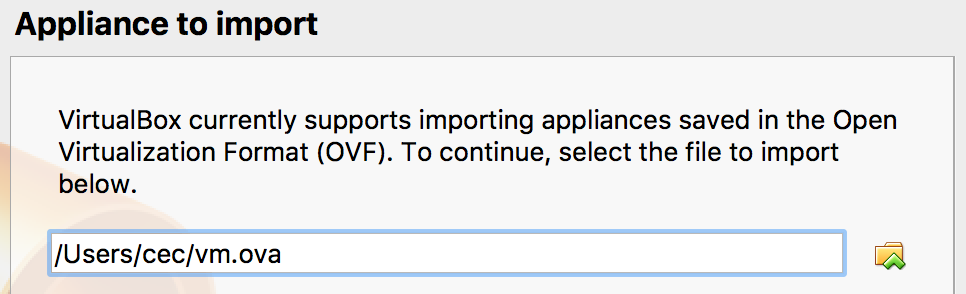
\includegraphics[width=\columnwidth]{img/vm1}
\end{figure}
\noindent
The image was prepared using VirtualBox 5.1.8. It has the following configuration: Ubuntu 16.04, 4 GB RAM, 10 GB hard drive, bridged network adapter with DHCP, US keyboard layout, GMT timezone.
\begin{figure}[H]
  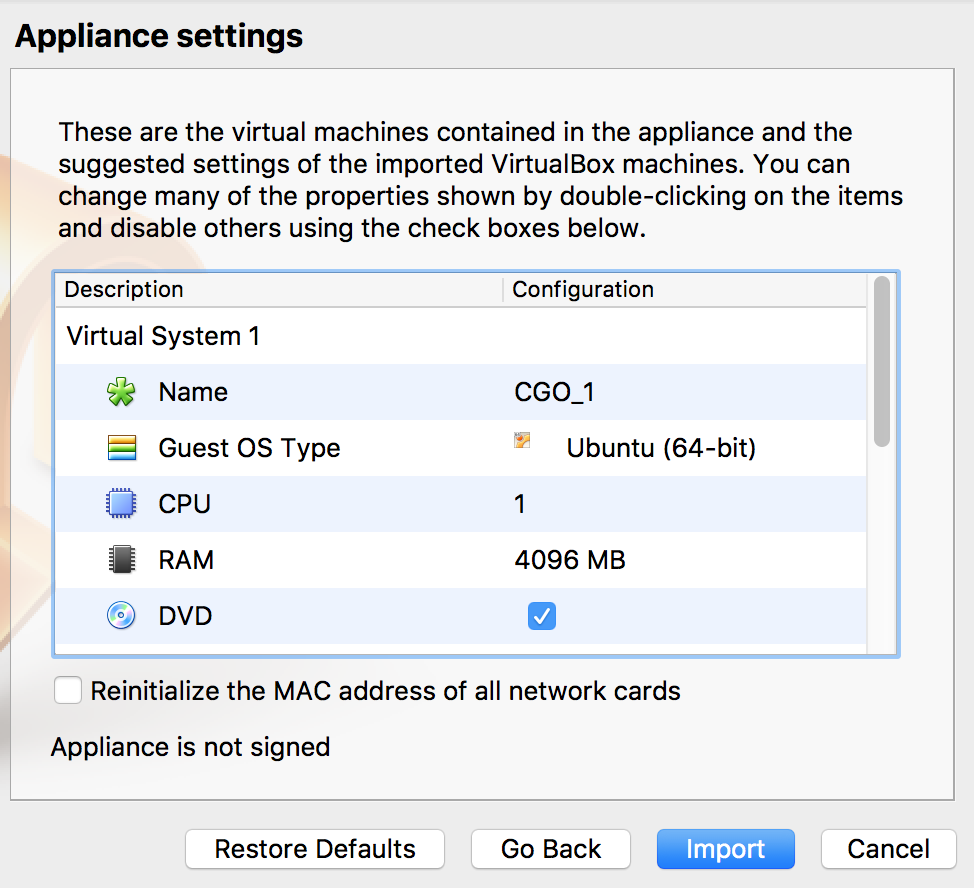
\includegraphics[width=\columnwidth]{img/vm2}
\end{figure}
\noindent
Start the machine and log in using username and password \texttt{cgo}. Once at the shell, run \texttt{launch}. This will start the Jupyter notebook server and print its address. You can access the notebooks at this address using the browser of the host device. Please note that the VirtualBox image does not have OpenCL, so new runtimes cannot be generated.

\subsubsection{Local Install}

See \url{http://chriscummins.cc/cgo17/} for instructions. Note that we only support Ubuntu 16.04 or OS X, and sudo privileges are required to install the necessary requirements. Other Linux distributions may work but will require extra steps to install the correct package versions.

% \subsubsection{Hardware dependencies}
%
% \subsubsection{Software dependencies}
%
% \subsubsection{Datasets}
%
% {\em Obligatory}

\clearpage
\subsection{Experiment Workflow}\label{subsec:workflow}

\begin{enumerate}
  \item Access the Jupyter notebook server using one of the three options described in Section~\ref{subsec:installation}.
  \item From the Jupyter server page, tick the checkbox next to one of the two notebooks: \texttt{AE.ipynb} for minimal artifact reproduction or \texttt{Paper.ipynb} for a comprehensive interactive paper.
  \item Click the button ``Duplicate''.
  \begin{figure}[H]
    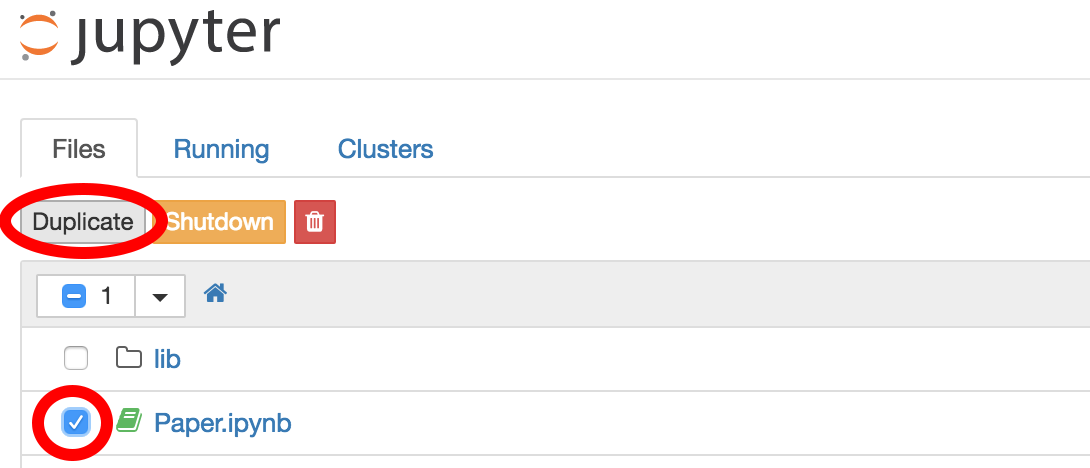
\includegraphics[width=\columnwidth]{img/notebook}
  \end{figure}
  \item Click on the name of the newly created copy, e.g. \texttt{Paper-Copy1.ipynb} or \texttt{AE-Copy3.ipynb}.
  \begin{figure}[H]
    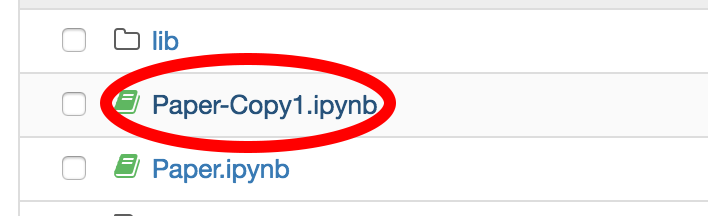
\includegraphics[width=\columnwidth]{img/notebook-copy}
  \end{figure}
  \item Repeatedly press the \emph{play} button (tooltip is ``run cell, select below'') to step through each cell of the notebook.
  
  OR select ``Kernel'' > ``Restart \& Run All'' from the menu to run all of the cells in order.
  \begin{figure}[H]
    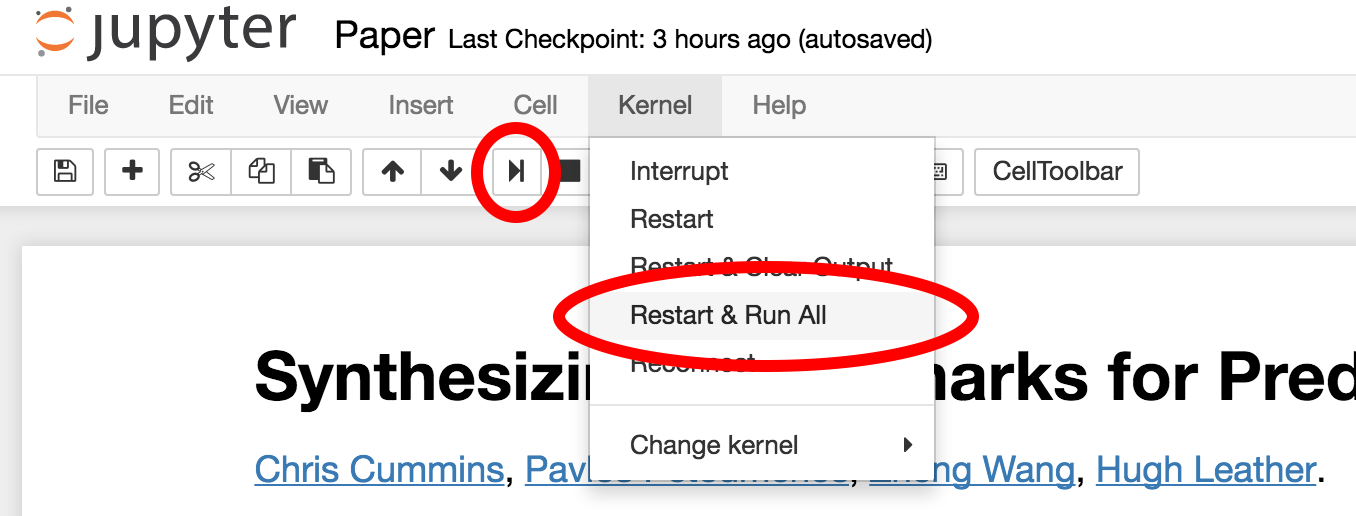
\includegraphics[width=\columnwidth]{img/jupyter}
  \end{figure}
\end{enumerate}


\subsection{Evaluation and Expected Result}

Each code cell within the Jupyter notebook generates an output. Expected results are described in text cells.

We include both the code necessary to evaluate the data used in the paper, and the code necessary to generate and evaluate new data. For example, we include the large neural network trained on all of the OpenCL on GitHub (which took 3 weeks to train), along with a small dataset to train a new one.

\newpage
\subsection{Experiment Customization}

The experiments are fully customizable. The Jupyter notebook can be edited ``on the fly''. Simply type your changes into the cells and re-run them. For example, in Table 1 of the \texttt{Paper.ipyn} notebook we cross-validate the performance of predictive models on an AMD GPU:

\begin{figure}[H]
  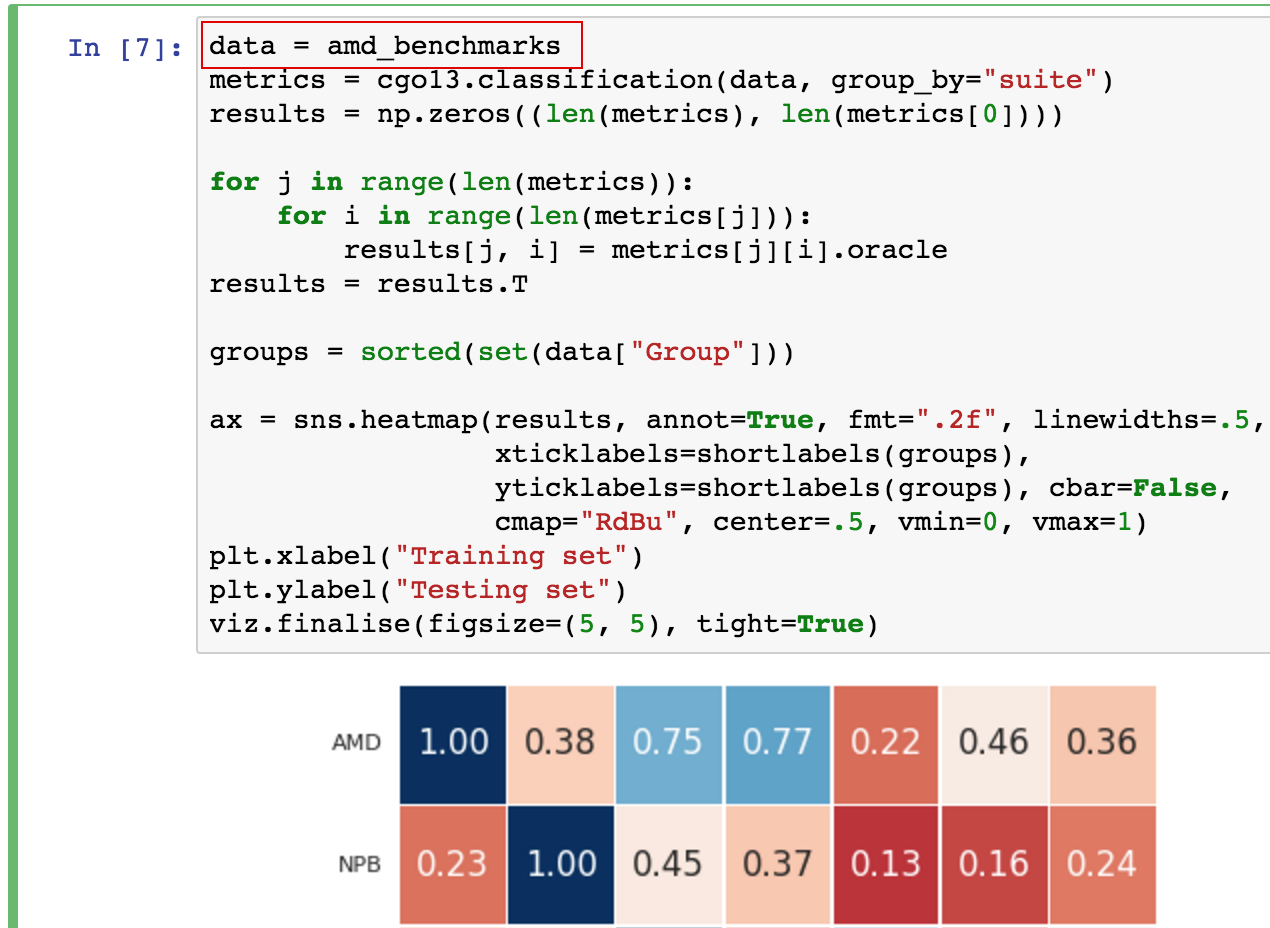
\includegraphics[width=\columnwidth]{img/example-1}
\end{figure}

\noindent
To replicate this experiment using the NVIDIA GPU, change the first line of the appropriate code cell to read \texttt{data = nvidia\_benchmarks} and re-run the cell:

\begin{figure}[H]
  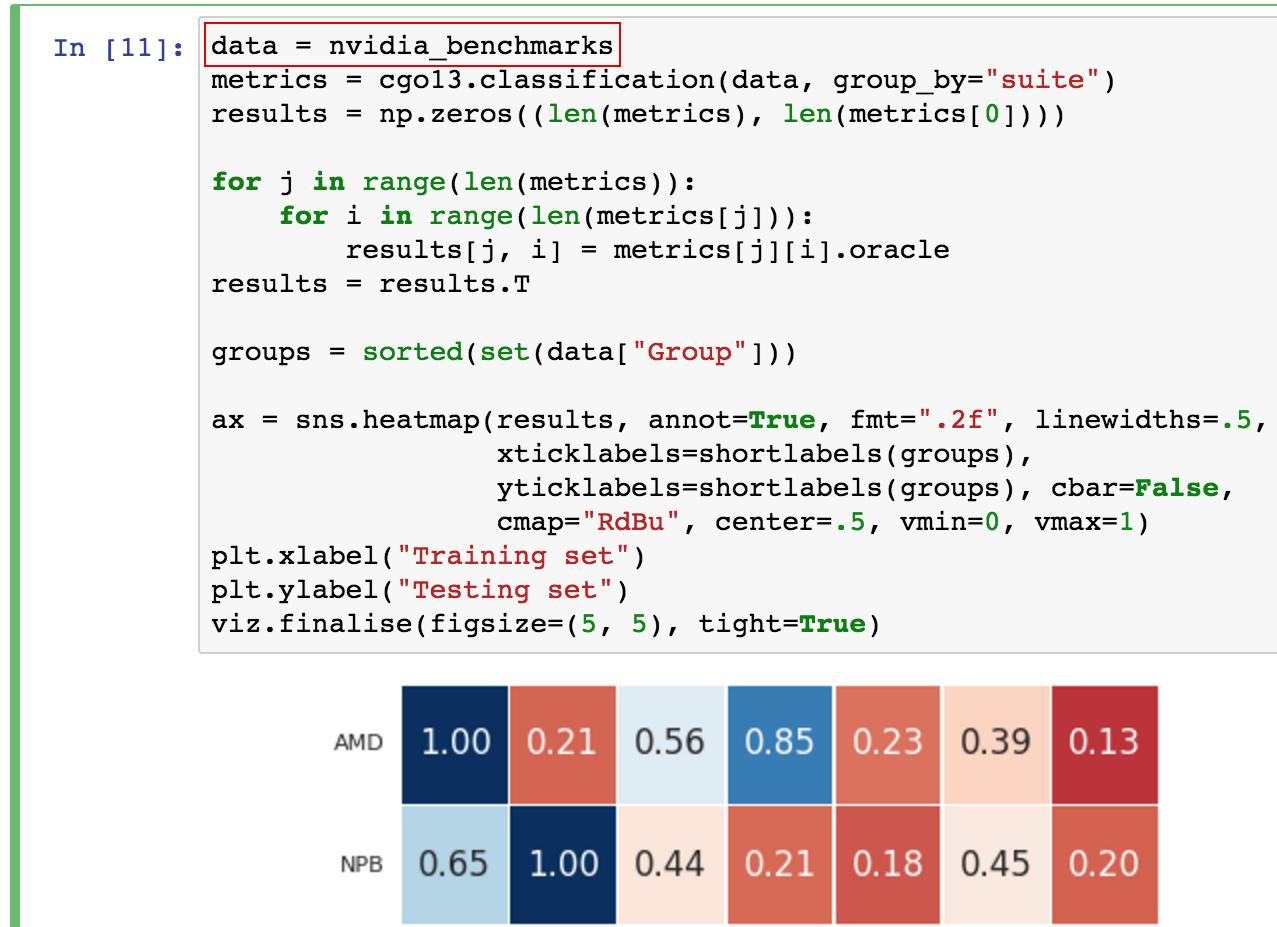
\includegraphics[width=\columnwidth]{img/example-2}
\end{figure}

\noindent
Note that some of the cells depend on the values of prior cells and must be executed in sequence.

CLgen has a documented API and command line interface. You can create new corpuses, train new networks, sample kernels, etc.


\subsection{Notes}
For more information about CLgen, visit:

\url{http://chriscummins.cc/clgen}

\noindent
For more information about Artifact Evaluation, visit:

\noindent
\url{http://ctuning.org/ae/submission-20161020.html}

% Fix rendering layout error introduced by flushend package:
\raggedend
